\documentclass[twoside]{article}
\usepackage{amssymb}
\usepackage{amsmath}
\usepackage{amsthm}
\usepackage{algorithm}
\usepackage{algpseudocode}
\usepackage{enumerate}% http://ctan.org/pkg/enumerate
\usepackage{pgfplots}
\usepackage{multicol}
\usepackage[hmarginratio=1:1,top=32mm,columnsep=20pt]{geometry}
\usepackage{fullpage}
\usepackage{pdflscape}
\usepackage{setspace}
\usepackage{tikz}
\usepackage[toc,page]{appendix}
\usepackage[shortlabels]{enumitem}\usepackage{draftwatermark}

\newcommand{\quotes}[1]{``#1''}

\theoremstyle{plain}% default
\newtheorem{theorem}{Theorem}[section]
\newtheorem{lemma}[theorem]{Lemma}
\newtheorem{proposition}[theorem]{Proposition}
\newtheorem*{corollary}{Corollary}

\theoremstyle{definition}
\newtheorem{definition}{Definition}[section]
\newtheorem{example}{Example}[section]
\newtheorem{exercise}[example]{Exercise}

\theoremstyle{remark}
\newtheorem*{rem}{Remark}
\newtheorem*{note}{Note}
\newtheorem{case}{Case}

\begin{document}
\parindent=0in
\parskip=12pt

\SetWatermarkText{Draft}
\SetWatermarkScale{5}

\title{
  Relative Probability on Finite Sample Spaces \\
  \large{
    SUBTITLE HERE
  }
}

\author{Max Sklar\\ Local Maximum Labs \\ DATE HERE}
\date{}

\maketitle
\thispagestyle{empty}

\begin{abstract}
This is an incomplete draft/outline of an upcoming paper. Please do not share
\end{abstract}

\tableofcontents
\newpage

\section{Introduction}

The mathematical foundations of probability theory are still very much open to debate!

Since Kolmogorov published the standard axioms for probability in 1933, there have been calls to relax or alter them for various applications. In Kolmogorov's Axiomatisation and Its Discontents\cite{lyon}, Lyon lays out these cases and their justifications. A question arises from this discuttion: can we discuss conditional probability when the condition event has probability zero? One would hope it not be forbidden to talk about the probability of an event given a hypothetical situation which will not occur\footnote{Another unintuitive feature of probability theory is that zero probability events do indeed occur, particularly when given a continuous distribution.}. Related to this question is whether we can talk about the relative probability of two events in a system, even though those two events may have probability zero.

The Kolmogorov model defines these values as a ratio of one probability to another. As a result, every time the indeterminate form \(\frac{0}{0}\) appears, the relative probability remains undefined. Undeterred by this state of affairs, mathematicians and engineers refer to this type of relative probability all the time. For example, if we consider the continuous probability distributrion over \([0, 1]\) given by the probability distribution function \(2x\), we know that the PDF at \(x = \frac{1}{2}\) is twice as much as the PDF at \(x = \frac{1}{4}\). In a sense, we believe that the former is twice as likely as the latter - even though we are only talking about \textit{probability density} or \textit{PDF} values.

Let us take the position that we may model probability in a non-standard way, and we can do so as long our new framework is logically consistent, and that the advertised applications correspond to the mathematical model\footnote{Lyon identifies this link between application and model as the bridge principle. A new set of axioms for probability could well give rise to a new and interesting mathematics, but if that mathematics cannot be linked to any application that anyone would reasonbly call probability, then it ought to go by a different name.}. Given the popularity of Bayesian methods as applied to machine learning in recent decades, and given that the methods used to search a hypothesis space in Bayesian inference relies on relative probability\cite{sklar_bias}, we ought to understand whether we can derive a framework for probability that takes the relationships between outcomes and events as fundamental.

This improves the Kolmogorov model - that takes absolute probability as fundamental - by both solving the conditional probability question and giving rise to new concepts and constructions to study.

\subsection{Goals}

We aim to demonstrate that a relative probability approach is not only viable, but has many properties that practicioners of all kinds will find attractive.

As a proof of this concept, we will construct a theory of relative probability on finite distributions. By omitting infinite distributions, we can temporarily set aside the concepts of measurable sets and countable additivity. This work will demonstrate that even with this vast simplification there is much to be learned. Relative probability requires a new set of fundamental rules and vocabulary to be a viable foundation, which we will construct.

These methods have applications in Bayesian statistics, even providing a new formulation of Bayes rule that is reflective of current practice. We will look at these applications of these ideas along with their algorithmic implementation.

Finally, we will discuss a critical feature of prelative probability functions, which is their ability to retain information when taking limits - for which absolute probability fails. In order to certify this feature, we delve into the topology and finish with a proof of compactness.

\section{Preliminaries}
\subsection{Magnitude Space}
\begin{definition}
The \textit{magnitude space} \(\mathbb{M}\) is the set of all positive real numbers, \(0\) and \(\infty\).
\[\mathbb{M} = [0, +\infty]\]
\end{definition}

Magnitudes roughly corresponding with our intuition of size.

\(\mathbb{M}\) is closed under addition with \(m + \infty = \infty\).

The products \(0 \cdot \infty\) and \(\infty \cdot 0\) are indeterminate. In all other cases, multiplication on \(\mathbb{M}\) is defined.

The multiplicative inverse \(m^{-1}\) is the defined on all \(\mathbb{M}\). We let \(0^{-1} := \infty\) and \(\infty^{-1} := 0\), even though it doesn't quite act as a multiplicative inverse in those cases.

The set of magnitudes is a totally ordered set under \(\leq\), meaning that for every two magnitudes either \(m_1 \leq m_2\) or \(m_2 \leq m_1\), and if both are true then \(m_1 = m_2\). The point at infinity can be considered a limit element, larger than all other magnitudes.

\subsection{The Wildcard Element}

\begin{definition}
Let the \textit{magnitude-wildcard space} \(\mathbb{M}^*= \mathbb{M} \cup \{\ast\}\) be the set of magnitudes along with a \textit{wildcard element}, \(\ast\).
\end{definition}

The wildcard element corresponds to several different concept, each appearing in a different type of practice:
\begin{itemize}
  \item The \textit{wildcard pattern} used in pattern matching and regular expressions in type theory and computer science
  \item The indeterminate form \(\frac{0}{0}\) in arithmetic.
  \item The standard \textit{NaN}, or \textit{Not a Number}\footnote{\quotes{Not a Number} may have been an unfortunate naming choice because it actually represents \textbf{any} number!} value in the IEEE standard for floating point arithmetic\cite{ieee}.
\end{itemize}

We define the following properties on \(\ast\) to allow addition and multiplication of any two magnitude-wildcard values.
\begin{enumerate}[(i)]
  \item \(0 \cdot \infty = \ast\)
  \item \(\ast + m = \ast\)
  \item \(\ast \cdot m = \ast\)
\end{enumerate}

Note that we now lose some basic properties of these operations. For example, we can no longer simplfy an expression like \(0x\) to \(0\). This will take some getting used to, but programmers familiar with the \textit{NaN} value in floating point arithmetic have long adapted to this adjustment.

\subsection{The Matching Relation}

\begin{definition}
The \textit{matching relation}\footnote{It helps to read \(:\cong\) as \quotes{is matched by}.} \(:\cong\) is a binary relation on \(\mathbb{M}^*\). \(m_1\) is matched by \(m_2\) when either \(m_1 = m_2\) or  \(m_2\) is the wildcard.
\[m_1 :\cong m_2 \Longleftrightarrow (m_1 = m_1) \vee (m_2 = \ast)\]
\end{definition}

We say that the left hand side of a matching relation is the \textit{parameter} and the right hand side is the \textit{constraint}. This reinforces the idea that the \(contraint\) may or may not contrain the parameter.

The following lemmas quickly follow from the definition.

\begin{lemma}
\label{wild_prop_1} If a magnitude matches a non-wildcard element, then the two values are equal. \[m_1 :\cong m_2 \wedge m_2 \neq \ast \Longrightarrow m_1 = m_2\]
\end{lemma}

\begin{lemma}
\label{wild_prop_2}
Every element is matched by the wildcard element. \(m :\cong \ast\)
\end{lemma}

\begin{lemma}
\label{wild_prop_3}
The wildcard element is matched only by itself. \(\ast :\cong m \Longrightarrow m = \ast\)
\end{lemma}

The matching relation asks if the parameter could be represented by the constraint. The wildcard element represents every single value, but it cannot be represented by any specific value. Alternatively, the wildcard element represents a loss of information about a parameter which can never be recovered. Hajek\cite{hajek} also calls these matching relations contraints, in that they may or may not bind the right hand side to a specific value.

The matching relation is reflexive and transitive, but unlike equality is not symmetric.

\begin{theorem}
The matching relation is transitive. In other words, for all \(m_1, m_2, m_3\) in \(\mathbb{M}\), if \(m_1 :\cong m_2\) and \(m_2 :\cong m_3\), then \(m_1 :\cong m_3\).
\end{theorem}

\begin{proof}
Assume that \(m_1 :\cong m_2\) and \(m_2 :\cong m_3\). If none of these values are the wildcards, then by property \ref{wild_prop_1}, they are all equal and \(m_1 :\cong m_3\). If \(m_1 = \ast\) then by property \ref{wild_prop_3}, \(m_2 = \ast\) and finally \(m_3 = \ast\) so the theorem holds. If \(m_2 = \ast\) then \(m_3 = \ast\) and \(m_1 :\cong m_3\) by property \ref{wild_prop_2}. And of course if \(m_3 = \ast\) alone, then by property \ref{wild_prop_2}, \(m_1\) is still matched by \(m_3\).
\end{proof}


\begin{theorem}
\label{theorem:matching_multiplication}
The matching relation preserves multiplication and addition. \(\forall a,b,a',b' \in \mathbb{M^*}\) if \(a :\cong a'\) and \(b :\cong b'\), then \(ab :\cong a'b'\) and \(a+b :\cong a'+b'\).
\end{theorem}

\begin{proof}
Let \(a,b,a',b' \in \mathbb{M^*}\), and let \(a :\cong a'\) and \(b :\cong b'\). If either \(a'\) or \(b'\) are wildcards, then \(a'b'\) is also a wildcard. If \(a'\) and \(b'\) are not wildcards, then \(a = a'\) and \(b = b'\), also making \(ab :\cong a'b'\). The same argument proves \(a+b :\cong a'+b'\).
\end{proof}

\section{Categorical Distribution}

Let \(\Omega\) be a set of mutually exclusive \textit{outcomes}. We assume that \(\Omega\) is finite so that we can count its members as \(|\Omega| = K\). We say there are \(K\) outcomes, or \textit{categories}.

\begin{definition}
A \textit{categorical distribution} on a \(\Omega\) is a function \(P: \Omega \rightarrow [0, 1]\) such that \(\sum_{h \in \Omega} P(h) = 1\)
\end{definition}

The set of all categorical distributions of size \(K\) can be embedded in \(\mathbb{R}^K\) as a (K-1)-dimentional object called a (K-1)-simplex. For example, if \(K = 3\), the resulting space of categorical distributions is an equilateral triangle embedded in \(\mathbb{R}^3\) connecting the points (1, 0, 0), (0, 1, 0), and (0, 0, 1).

Because the set of categorical distributions is embedded in \(\mathbb{R}^K\), its topological properties are well understood. The simplex is closed, bounded, and compact. Practically, this means that any sequnce of points on the simple will converge to one or more points on the simplex allowing both pure and applied practicioners to talk about limit and boundary conditions.

Because we are talking about absolute probability, relative information is lost at the boundaries. For example, if \(\Omega = {a, b, c}\) with \(P(a) = 1\) and \(P(b) = P(c) = 0\), we cannot compare the probabilities of \(b\) and \(c\) as we can in the rest of the simplex.

\subsection{Events}

An \textit{event} is a set of outcomes. We define \(\mathcal{F}\) as the space of all possible events. \(\mathcal{F}\) is the power set\footnote{In general, \(\mathcal{F}\) is not the entire power set of \(\Omega\) but typically is when \(\Omega\) is finite. We need not concern ourselves with the \(\sigma\)-algebra of measurable sets here.} of \(\Omega\), meaning that \(\mathcal{F} = \mathcal{P}(\Omega)\), and for any subset \(e \subseteq \Omega\), \(e \in \mathcal{F}\).

In the previous section, we defined the probability of individual outcomes. We can now define the probability function on events instead of outcomes. Definiting probability on the event level rather than the outcome level is a curcial insight in the development of probability theory (and measure theory more generally). Even though the process is far simpler for finite distributions, we must pay attention to this layer in order for the framework to generalize.

For all \(e\) in \(\mathcal{F}\),
\[ P(e) = \sum_{h \in e}{P(h)}\]

We can take \(P\) as acting either on outcomes or events using the convention \(P(h) = P(\{h\})\).

\(\Omega\) itself the \textit{universal event} of all outcomes, with probability 1.

\[P(\Omega) = \sum_{h \in \Omega}{P(h)} = 1\]

\subsection{Relative Probability Function}
\label{section:standard_relative_prob}

A \textit{relative probability function}, or \textit{RPF}, measures the probability of one event with respect to another. For example, we may wish to talk about an event that is \quotes{twice as likely} as another, even if we don't know the absolute probability of either event.

We continue to use P to represent the RPF but with two inputs instead of one. The expression \(P(e_1, e_2)\) can be read as the probability of \(e_1\) relative to \(e_2\).

\[P: \mathcal{F} \times \mathcal{F} \rightarrow \mathbb{M}^*\]

We define relative probability in terms of absolute probability as a ratio, in the style of the standard Kolmogorov framework.

\begin{definition}
\label{def:ratio}
The relative probability of events \(e_1\) and \(e_2\) on an categorical distribution \(P\) is given as
\[P(e_1, e_2) = \frac{P(e_1)}{P(e_2)}\]
\end{definition}

If \(P(e_1) = p(e_2) = 0\), then \(P(e_1, e_2) = \ast\), representing the classical problem of zero-probability events being incomparable.

\begin{theorem}
For all events \(e_1, e_2, e_3\), \(P(e_1, e_3) :\cong P(e_1, e_2) \cdot P(e_2, e_3)\)
\end{theorem}

\begin{proof}
Start with the case that \(e_2 \neq 0\). Then \(P(e_1, e_2) \cdot P(e_2, e_3) = \frac{P(e_1)}{P(e_2)}\frac{P(e_2)}{P(e_3)} = \frac{P(e_1)}{P(e_3)} = P(e_1, e_3)\). When \(e_2 = 0\), \(P(e_1, e_2) \cdot P(e_2, e_3) = \frac{P(e_1)}{P(e_2)}\frac{P(e_2)}{P(e_3)} = \ast\). Because \(\ast\) matches everything, then the matching statement holds. Because it holds in both cases, the theorem is true.
\end{proof}

\section{Relative Categorical Probability Functions}
\label{section:new_relative_prob}

In section \ref{section:standard_relative_prob}, the relative probability function was derived from the absolute probability function. Here in section \ref{section:new_relative_prob}, we start with the relative probability function as the fundamental object of study.

Consider a relative probability function \(P\) that acts on outcomes only.

\begin{definition}
\label{def:fundamental_laws}
Let \(\Omega\) be the set of outcomes, and \(P: \Omega \times \Omega \rightarrow \mathbb{M}^*\) be a function acting on two outcomes to product a magnitude-wildcard. \(P\) is a \textit{relative probability function on the outcomes of \(\Omega\)} if it obeys the following \textit{3 fundamental axioms of relative probability}:

\begin{enumerate}[(i)]
\item The \textit{identity axiom}: \(P(h, h) = 1\)
\item The \textit{inverse axiom}: \(P(h_1, h_2) = P(h_2, h_1)^{-1}\)
\item The \textit{composition axiom}: \(P(h_1, h_3) :\cong P(h_1, h_2) \cdot P(h_2, h_3)\)
\end{enumerate}

\end{definition}

If \(P\) is such a relative probability function, \(P(h_1, h_2)\) can be read as the probability of \(h_1\) relative to \(h_2\).

Let us pause for a moment to discuss how these axioms where chosen. There are several questions that one must ask when developing a set of axioms.

One class of questions concerns the scope of the axioms. Do the laws correspond precisely with the concept at hand? Do they encompass every instance of the concept that one might want to study? Do they allow for any possibilities that should not be considered? This process not only involves playing with the axioms themselves, but also refining the concept they are meant to conjure up. This involves strengthening and weaking the axioms until they fit.

The second class concerns the design of the axioms. Are all of them required or is one a consequence of the others? Are they organized in a useful way to the people who will use them?

[MORE ON THIS]

\subsection{From Outcomes to Events}

Our next task is to upgrade \(P\) to operate on the event level. In definition \ref{def:ratio}, the relative probability of two events were the ratio of their absolute probabilities. Because we no longer have access to absolute probability, the best we can do is measure it relative to a \textit{reference outcome} \(h^*\). Because this ratio might be indeterminate, we use the matching relation instead of equality.

For all \(h^* \in \Omega\),

\begin{equation}
\label{eq:event_def_ratio_match}
P(e_1, e_2) :\cong \frac{\sum_{h_1 \in e_1} P(h_1, h^*)}{\sum_{h_2 \in e_2} P(h_2, h^*)}
\end{equation}

In addition, we require that \(P\) obeys the 3 fundamental laws of relative probability in Definition \ref{def:fundamental_laws}. Finally, if a relative probability is not constrained by any of these requirements, then it remains a wildcard.

These requirements may seem reasonable, but how can we know for sure that they provide a complete and consistent definition of \(P: \mathcal{F} \times \mathcal{F} \rightarrow \mathbb{M}^*\)? The following must be shown:

\begin{enumerate}[(i)]
  \item \label{event_def_proof_1} If two distinct values for \(h^*\) in statement \ref{eq:event_def_ratio_match} yield non-wildcard constraints on \(P\), then they must be equal.
  \item \label{event_def_proof_2} The constraint in \ref{eq:event_def_ratio_match} will not violate the axioms of identity, inverse, or composition.
\end{enumerate}

Proof of \ref{event_def_proof_1}

Let \(h_1^*\) and \(h_2^*\) be two distinct values for \(h^*\) in \ref{eq:event_def_ratio_match}, and neither causes the ratio to be a wildcard. Then we want to check that

\begin{equation}
\label{eq:relative_event_unique}
\frac{\sum_{h_1 \in e_1} P(h_1, h_1^*)}{\sum_{h_2 \in e_2} P(h_2, h_1^*)} = \frac{\sum_{h_1 \in e_1} P(h_1, h_2^*)}{\sum_{h_2 \in e_2} P(h_2, h_2^*)}
\end{equation}

None of the terms above can be wildcards, because it would cause the whole expression to be a wildcard. The key to this argument is in looking at the value of \(P(h_1^*, h_2^*)\). Fortunately, we can start by eliminating \(P(h_1^*, h_2^*) \notin \{0, \infty, \ast\} \)

Suppose \(P(h_1^*, h_2^*) = \ast\). Then for all \(h\), \(P(h_1^*, h_2^*) = \ast :\cong P(h_1^*, h) \cdot P(h, h_2^*)\). By matching property \ref{wild_prop_3}, this means that \(P(h_1^*, h) \cdot P(h, h_2^*) = \ast\), and therefore at least one of those terms is \(\ast\). But looking back on equation \ref{eq:relative_event_unique}, this means that if there are any terms at all in these sums, at least one of them must be \(\ast\), contradicting our assumption. And if there happen to be no terms in this equation then both sides are \(\frac{0}{0}=\ast\). So \(P(h_1^*, h_2^*) \neq \ast\)

Perhaps \(P(h_1^*, h_2^*) = 0\). Then, every term from equation \ref{eq:relative_event_unique} of the form \(P(h_1, h_2^*)\), we have \(P(h_1, h_2^*):\cong P(h_1, h_1^*) \cdot P(h_1^*, h_2^*) = P(h_1, h_1^*) \cdot 0\). Then either \(P(h_1, h_2^*) = 0\) or \(P(h_1, h_1^*) = \infty\). More generally, equation \ref{eq:relative_event_unique}, this means that every term in equation \ref{eq:relative_event_unique} is either \(0\) or \(\infty\) and its analogous term on the opposite side is the inverse.

Looking at the sums as a whole, each sum is made up either entirely of 0s or contains an \(\infty\) in which case the sum is \(\infty\).

[ GOTTA FILL THIS IN ]

By an analogous argument  \(P(h_1^*, h_2^*) \neq \infty\)

So now we can assume that \(P(h_1^*, h_2^*) \notin \{0, \infty, \ast\} \). The allows us to multiply the left hand side of equation \ref{eq:relative_event_unique} by \(1 = \frac{P(h_1^*, h_2^*)}{P(h_1^*, h_2^*)}\) and distribute into the sum to get:

\[\frac{\sum_{h_1 \in e_1} P(h_1, h_1^*) \cdot P(h_1^*, h_2^*)}{\sum_{h_2 \in e_2} P(h_2, h_1^*) \cdot P(h_1^*, h_2^*)} = \frac{\sum_{h_1 \in e_1} P(h_1, h_2^*)}{\sum_{h_2 \in e_2} P(h_2, h_2^*)}\]

Note that the simplification with the transitive rule needs to be justified in the wildcard space. We can be sure that none of the terms \(P(h_1, h_1^*)\) or \( P(2_1, h_1^*)\) are \(\ast\) because that would make the entire expression \(\ast\) which contradicts our assumption. Because \(P(h_1^*, h_2^*)\) is a magnitude between 0 and \(\infty\), we can be sure that the transitive simplification holds.

Proof of \ref{event_def_proof_2}

Starting with the identity axiom:

\[P(e_1, e_1) :\cong \frac{\sum_{h_1 \in e_1} P(h_1, h^*)}{\sum_{h_1 \in h_2} P(h_1, h^*)}\]

The constraint - being the ratio of two identical terms - is either 1 or \(ast\) in the case that the sums are \(0\) or \(\infty\). Therefore, there cannot be a contradiction to \(P(e_1, e_1) = 1\)

The inverse property...
The composition property on the event level is \(P(e_1, e_3) :\cong P(e_1, e_2) \cdot P(e_2, e_3)\)

FILL IN

\begin{theorem}
Given events \(e_1\) and \(e_2\) where \(e_1 \cup e_2 \neq \varnothing\), we have \[P(e_1, e_2) = \sum_{h_1 \in e_1} \frac{1}{\sum_{h_2 \in e_2} p(h_2, h_1)}\].
\end{theorem}

\begin{proof}
FILL IN
\end{proof}

We then derive the absolute probability function as

\[P(e) = P(e, \Omega) = \sum_{h \in e} \frac{1}{\sum_{h' \in \Omega}p(h', h)}\]

\subsection{Degenerate Cases}

Suppose that \(K = 0\). Then \(\Omega\) is empty, and there are no outcomes. Surprisingly, there is still an RPF because of the event represented by the empty set \(\varnothing\). In this case \(P(\varnothing, \varnothing) = 1\) is the only RPF. This is a mathematical by product of our definition, but an interesting comparison to the case of absolute distributions where such a function does not exist (because with no outcomes, they cannot sum to 1).

Now we let \(K = 1\), and \(\Omega = {h}\). There is still only a single, trivial RPF P, where \(P(h, h) = 1\), and \(P(\varnothing, h) = 0\). This matches the absolute case where the probability of the single outcome must be 1.

\section{New Concepts for Relative Probability}

We have successfully defined the relative probability function in section \ref{section:new_relative_prob}, and we can construct examples. However, because we now allow zero probability outcomes and events to be assigned relative values, new situations arise that do not occur in the standard model. We therefore need some new vocabulary to talk about these situations. These include whether events are comparable or possible relative to each other, and how that affects the structure of the RPF.

\subsection{Matching and Comparability}

If an RPF assigns \(\ast\) to the two events, then it has lost information about the relationship between those two events.

\begin{definition}
Events \(e_1\) and \(e_2\) are \textit{comparable} if \(P(e_1, e_2) \neq \ast\).
\end{definition}

\begin{definition}
A relative probability function is \textit{totally comparable} if every pair of events are comparable.
\end{definition}

A totally comparable RPF has the maximum amount of information filled in about the relative probability of two events. Some RPFs may have less information but nevertheless are consistent with RPFs that have more. The following definition encapulates this relationship.

\begin{definition}
Let \(P_1\) and \(P_2\) be relative probability functions. \(P_1\) is matched by \(P_2\) if and only if all of relative probabilities of \(P_1\) are matched by those of \(P_2\).
\[\forall e_1, e_2 \in \mathcal{F}, P_1(e_1, e_2) :\cong P_2(e_1, e_2)\]
\end{definition}

\begin{theorem}
Let \(P_1\) and \(P_2\) be relative probability functions on \(\Omega\) where \(P_1 :\cong P_2\) and \(P_2\) is totally comparable. Then, \(P_1\) and \(P_2\) must be equal.
\end{theorem}

\begin{proof}
Assume that \(P_1 :\cong P_2\) and choose any two events, \(e_1\) and \(e_2\). By definition, it directly follows that \(P_1(e_1, e_2) :\cong P_2(e_1, e_2)\). Because \(P_2\) is totally comparable, \(P_2(e_1, e_2) \neq \ast\). By matching property \ref{wild_prop_3}, this means that \(\ast :\ncong P_2(e_1, e_2)\). This in turn means, that \(P_1(e_1, e_2) \neq \ast\) because if it were then it would not be matched by \(P_2(e_1, e_2)\). Since neither expression is a wildcard, using matching property \ref{wild_prop_1} we conclude that \(P_1(e_1, e_2) = P_2(e_1, e_2)\). Therefore, these two RPFs are equal on all possible inputs.
\end{proof}

\begin{theorem}
Every RPF is matched by an absolute probability function
\end{theorem}

\begin{proof}
FILL IN
\end{proof}

\begin{theorem}
An absolute probability function is totally comparable if and only if at most 1 outcome is assigned 0 probability.
\end{theorem}

\begin{proof}
Let P be an (absolulte) probability function, with \(h_1\) and \(h_2\) being two outcomes. If \(P(h_1) = P(h_2) = 0\), then the relative function (CITE) \(P(h_1, h_2) = \frac{0}{0} = \ast\), and thus P is not totally comparable. If only outcome \(h_1\) is assigned 0, then \(P(h_1, h_1) = 1\), \(P(h_1, h_2) = 0\), and \(P(h_2, h_1) = \infty\). Any other pairing that does not involve \(h_1\) will be the quotient of two positive numbers, and thus also comparable. Therefore, P is comparable if only 1 outcome is assigned 0 probability.
\end{proof}

\subsection{Possibility Classes}

\begin{definition}
Events \(e_1\) and \(e_2\) are \textit{mutually possible} if they are comparable and \(0 < P(e_1, e_2) < \infty\).
\end{definition}

\begin{theorem}
The relationship of mutually possible events is an \textit{equivalence relation}, being reflexive, symmetric and transitive.
\end{theorem}

\begin{proof}
For reflexive, \(P(e_1, e_1) = 1\), so every event is comparable to itself.

For symmetric, \(P(e_1, e_2) = P(e_2, e_1)^{-1}\), which means that each can be in \(\{0, \infty, \ast\}\) if and only if the other one is as well.

For transitive, we use the composition axiom which states that \(P(e_1, e_3) :\cong P(e_1, e_2) \cdot P(e_2, e_3)\). If the last 2 values are positive real numbers, then their product is also a positive real number and equal to \(P(e_1, e_3)\).
\end{proof}

\begin{definition}
The event \(e_1\) is \textit{impossible} with respect to \(e_2\) if \(P(e_1, e_2) = 0\). The event \(e_1\) is \textit{possible} with respect to \(e_2\) if they are comparable and \(P(e_1, e_2) > 0\)
\end{definition}

\begin{theorem}
The relationship of being possible is a \textit{preorder}, or in other words both reflexive and transitive.
\end{theorem}

\begin{proof}
It must be reflexive because \(P(e, e) = 1\). If \(P(e_1, e_2) > 0\) and \(P(e_2, e_3) > 0\) then their product is also greater than zero, and by the fundamental property, equal to \(P(e_1, e_3)\) thus making it transitive.
\end{proof}

If we consider a possibility relationship with respect to the equivalence classes of mutually possibility, then we have a partial order.

The theorems above can be summerized as follows. Given any two events, \(e_1\) and \(e_2\), exactly one these is true.
\begin{enumerate}[(i)]
  \item \(e_1\) and \(e_2\) are mutually possible.
  \item \(e_1\) is impossible with respect to \(e_2\).
  \item \(e_2\) is impossible with respect to \(e_1\).
  \item \(e_1\) and \(e_2\) are not comparable.
\end{enumerate}

\begin{theorem}
If an RPF is totally comparable, then the equivalance classes of mutually possible events are \textit{totally ordered}. That is, each member of an equivalence class of events is comparable to each member of another class with that comparison always being 0 or always being \(\infty\).
\end{theorem}

\begin{proof}
FILL IN
\end{proof}

\subsection{Totally Mutually Possible RPFS}

\begin{definition}
A relative probability function is called \textit{totally mutually possible} if all of its outcomes\footnote{Note that this applies to individual outcomes and not events. The empty event \(e = \{\}\) will be impossible with respect to any outcome.} are mutually possible. Mutually possible RPFs satisfy \textit{Cromwell's rule} in Bayesian inference, which states that prior beliefs should assign probability zero or one to events\footnote{It would be stated differently in continuous space of course.}.
\end{definition}

\begin{theorem}
A totally mutually possible RPF can be represented by an absolute probability function \(P: \Omega \rightarrow (0, 1)\) which contains no zero-probability events.
\end{theorem}

\begin{proof}
Define the absolute probability of outcome \(h\) as \(P(h, \Omega)\). By definition of relative probability on events we have for every outcome \(h^*\):

\[P(h)=P(h, \Omega):\cong \frac{P(h, h^*}{\sum_{h_1 \in \Omega} P(h_1, h^*)}\]

Now let \(h^* = h\)

\[P(h):\cong \frac{P(h, h)}{\sum_{h_1 \in \Omega} P(h_1, h)}=\frac{1}{\sum_{h_1 \in \Omega} P(h_1, h)}\]

Because \(P\) is totally mutually possible, \(P(h_1, h)\) will always be a value \(\notin \{0, \infty, \ast\). Therefore, the sum is the same and each \(P(h)\) is non-zero. This means that all of the relative probabilities \(P(h_1, h_2)\) will have to equal the ratio \(\frac{P(h_1)}{P(h_2}\). Therefore, the absolute probability function contains all the information needed to construct the relative probability function without loss of information.
\end{proof}

\section{Composing Relative Probability Functions}

Let \(P_0, P_1, ..., P_{K-1}\) be relative probability functions. Each of these probability functions have unique categories in their own right.

Let the set of outcomes acted upon by \(P_k\) be \(\Omega_k\), so that \(P_k: \Omega_k \times \Omega_k \rightarrow \mathbb{M}^{\ast}\). We take all \(\Omega_k\) to be disjoint from one another.

We can combine all of these relative probability functions together with a top level probability function \(P_\top\)\footnote{Pronounced \quotes{P-Top}.} with outcome space \(\Omega_\top = \{\Omega_0, \Omega_1, \Omega_2, ... \Omega_{K- 1}\}\).

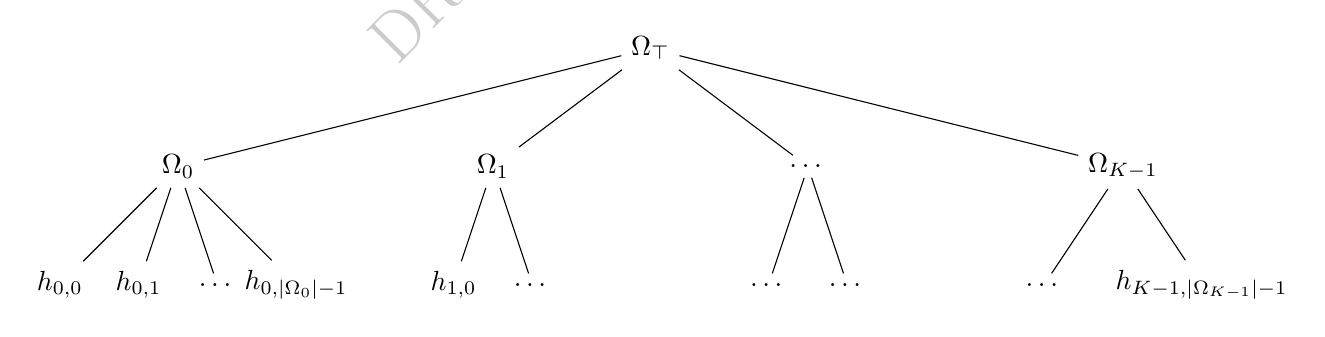
\begin{tikzpicture}
\node {\(\Omega_\top\)} [sibling distance = 4cm]
  child {node {\(\Omega_0\)}  [sibling distance = 1cm]
    child {node {\(h_{0, 0}\)}}
    child {node {\(h_{0, 1}\)}}
    child {node {\dots}}
    child {node {\(h_{0, |\Omega_0| - 1}\)}}
  }
  child {node {\(\Omega_1\)}  [sibling distance = 1cm]
    child {node {\(h_{1, 0}\)}}
    child {node {\dots}}  
  }
  child {node {\dots}  [sibling distance = 1cm]
    child {node {\dots}}
    child {node {\dots}}
  }
  child {node {\(\Omega_{K-1}\)}   [sibling distance = 2cm]
    child {node {\dots}}
    child {node {\(h_{K-1, |\Omega_{K-1}| - 1}\)}}
  };
\end{tikzpicture}

Now let \(\Omega\) be the set of all outcomes \(\Omega_0 \cup \Omega_1 \cup \dots \Omega_{K-1}\). We can create a new RPF - just called \(P\) acting on \(\Omega\) - with the following assumptions:

1) If the two outcomes fall under the same component, then their relative probabilities do not change:

\begin{equation}
\label{rpf_composition_same_branch}
P(h_{k, i}, h_{k, j}) = P_k(h_{k, i}, h_{k, j})
\end{equation}

2) If the two outcomes fall under different components, then their relative probabilities are given as follows.

\begin{equation}
\label{rpf_composition_different_branch}
P(h_{k_1, i}, h_{k_2, j}) = P_{k_1}(h_{k_1, i}, \Omega_{k_1}) \cdot  P_{\top}(\Omega_{k_1}, \Omega_{k_2}) \cdot P_{k_2}(\Omega_{k_2}, h_{k_2, j})
\end{equation}

Note the use of the composition property to traverse up and down the tree. One could of course imagine this for a tree of many levels, and each level having variable height.

\begin{theorem}
\(P\) respects the fundamental property.
\end{theorem}

\begin{proof}
Identity is obvious because an outcome is on the same component as itself, meaning that we can use equation \ref{rpf_composition_same_branch} to get \(P(h_{k, i}, h_{k, i}) = P_k(h_{k, i}, h_{k, i}) = 1\)

[Add Inverse ]

Composition is also obvious if all of the values are in the same component as it reduces to the transitive property within that component.

[Add Composition for different components]
\end{proof}

\begin{theorem}
\(P\) is totally comparable if and only if the following are true:

\begin{enumerate}
\item \(P_{\top}\) is totally comparable
\item For all \(k \in \{0, 1, ..., K - 1\}\), \(P_k\) is totally comparable
\item There is at most one component with outcomes that are impossible with respect to that component. Equivalently, if \(h_{k_1, i}\) and \(h_{k_2, j}\) are two components, and \(P_{k_1}(h_{k_1, i}) = P_{k_2}(h_{k_2, j}) = 0\), then \(k_1 = k_2\). Also equivalently, all components except at most one are totally mutually possible.
\end{enumerate}
\end{theorem}

\begin{proof}
FILL IN (both directions)
\end{proof}

\section{Bayesian Inference on Relative Distributions}

A relative probability function represents a belief over the set of potential hypotheses in \(\Omega\).

Start with the traditional Bayesian formula for conditional probability for \(h \in \Omega\) assuming that we recieve data \(D\).

\[P(h|D) = \frac{P(D|h) \cdot P(h)}{P(D)}\]

Now we are going to consider relative probability by looking at the ratio between two hypotheses.

\[\frac{P(h_1|D)}{P(h_2| D)} = \frac{P(D|h_1) \cdot P(h_1)}{P(D)} \div \frac{P(D|h_2) \cdot P(h_2)}{P(D)} = \frac{P(D|h_1) \cdot P(h_1)}{P(D|h_2) \cdot P(h_2)} \]

Next make the following subsitutions:

For the ratio of absolute distributions, subsitute the relative distribution: \(\frac{P(h_1)}{P(h_2)} \rightarrow P(h_1, h_2) \)

For the ratio of posterior distributions, subsitute the relative posterior: \(\frac{P(h_1|D)}{P(h_2|D)} \rightarrow P(h_1, h_2|D) \)

The liklihood ratio: \(\frac{P(D|h_1)}{P(D|h_2)} \rightarrow P(D|h_1, h_2) \)

Now we get bayes rule for relative probability:

 \[P(h_1, h_2|D) = L(D|h_1, h_2) P(h_1, h_2)\]
 
 The likelihood ratio \(L(D|h_1, h_2)\) is essentially a description of how the different hypotheses rate the likelihood of data. It is also a relative probability in its own right, and must obey the fundamental properties (cite).
 
 Therefore, the act of bayesian inference is an element-by-element multiplication of two different RPFs \(L(D|h_1, h_2)\) and \(P(h_1, h_2)\). We show that the product of two RPFs obeys the fundamental properties.

\begin{theorem} 
Let \(P_1\) and \(P_2\) be relative probability functions on \(\Omega\). Define \(P(h_1, h_2) = P_1(h_1, h_2) \cdot P_2(h_1, h_2)\). Then, \(P\) is also an RPF, that it is obeys the fundamental properties.
\end{theorem}

\begin{proof} 
Use the multiplication property of the matching relation in equation \ref{theorem:matching_multiplication}.
 
Identity: \[P(h_1, h_1) = P_1(h_1, h_1) P_2(h_1, h_1)=1 \cdot 1=1\]
 
Inverse: \[P(h_1, h_2) = P_1(h_1, h_2) \cdot P_2(h_1, h_2)=P_1(h_2, h_1)^{-1} \cdot P_2(h_2, h_1)^{-1}=(P_1(h_2, h_1) \cdot P_2(h_2, h_1))^{-1}=P(h_2, h_1)^{-1}\]
 
Composition: \[P(h_1, h_2)P(h_2, h_3)=P_1(h_1, h_2) P_2(h_1, h_2)P_1(h_2, h_3) P_2(h_2, h_3) :\cong P_1(h_1, h_3) P_2(h_1, h_3)=\]
\end{proof}

\begin{theorem}
Once two outcomes become uncomparable, they will never be comparable again. In other words, if \(P(h_1, h_2)=\ast\), then \(P(h_1, h_2|D) = \ast\).
\end{theorem}

\begin{proof}
\(P(h_1, h_2|D) = L(D|h_1, h_2) P(h_1, h_2) = L(D|h_1, h_2) \cdot \ast = \ast\)
\end{proof}

\begin{theorem}
Once an outcome becomes impossible with respect to another event, it will either remain impossible or become uncomparable. In other words,  if \(P(h_1, h_2)=0\), then \(P(h_1, h_2|D) \in {0, \ast}\).
\end{theorem}

\begin{proof}
\(P(h_1, h_2|D) = L(D|h_1, h_2) P(h_1, h_2) = L(D|h_1, h_2) \cdot 0\). Normally, this would simplify to 0, but with the matching relation in \(\mathbb{M}^*\), this will be \(\ast\) if \(L(D|h_1, h_2) \in {\infty, \ast}\).
\end{proof}

\section{Implementation}

Finally, we implement relative probabiliy as a python class as a demonstration of its usage and relevance.

How to implement this in code, and point to open source example.

Note the connection between magnitude space and the extended real number line, which we can implement through floating point numbers.

This can be implemented by storing K values.

For each category, we have a tier. Items in the same tier are comparable. Each Tier has a parent tier, where items in this teir are said to be impossible relative to anything in its ancestor tiers.

For each category, we also store a floating point number called the value, which should be taken as the log of an unnormalized probability. Note that we will not allow inf or NaN here.

Get the relative probability of 2 categories. Algorithm: If they are in the same tier, then subtract their values and take the exp. If they are in different tiers, do a graph search on the tier. If the first is < the second, the answer is 0. If the first is > the second, the answer is 1. And if they are uncomparable, then the answer is Wildcard, NaN.

Generate and indifferent distribution of category K. Algorithm: Create a single tier where all values are set to 0.

Change the relative probability of item \(k_1\) with respect to \(k_2\), and set it to \(q\). Algorithm: UNSURE

Set the probability \(k_1\) to some absolute value with respect to either the whole distribution, or to its tier.

Randomly sample from this distribution. Algorithm: Only look at the top tier.

Randomly sample from this distribution, but remove certain categories. Algorithm: If the top tier categories are gone, look to see if a top tier remains. If there are multiple top tiers, then there's no way to do it!

Ask: Is this distribution totally mutually possible? Algorithm: Look are a single top tier.

Ask: Is it totally mutually comparable? Algorithm: Look for a linear list of tiers.

\section{Topology of Relative Probability Spaces}

The idea of a limit distribution requires particularly around the idea of limits. Mathematics can be great at modelling the real world even if it's ideas are theoretically impossible. For example, we might believe that it is impossible for a certain natural process to repeat an infinite number of times, and yet we may still take its value to be infinity in order to get some kind of bound on what that system will look like in the long run. Likewise, it still makes sense to consider a particular outcome in a probabilistic system as certain while maintaining information about the other outcomes in order to calculate the effects of such a limit. [CLEAN UP WORDING OF PARAGRAPH] To this end, we will prove that the space of fully comparable relative distributions is compact.

TODO: Warn people that background in topology is required for this section, and then we can shorten it up! Also, this section can be skipped if not interesting.

One of the benefits of relative probability spaces is their properties with respect to limits. Specifically, if we look at the space of (absolute) categorical distributions on \(\Omega\) and we allow the probability of one outcome to approach 1, then all of the other probabilities will be forced down to 0 and become incomparable with one another. In the relative probability space, the information about the ratios of probabilities of the other outcomes can be preserved even as a single outcome reaches a probability of 1.

If the space of totally comparable RPFs can be shown to be compact, then we know that relative probabilites of outcomes and events are preserved even as they both approach zero relative to another event.

In order to prove compactness, we first must define a topology on the space of totally comparable RPFs. This means identifying the sets that are open (or intuitively, sets that fully surround all of it's members and don't contain its boundary). This starts with finding a \textit{basis of open sets} from which all other open sets can be constructed through countable unions.

For the absolute probability function, we can use \(K-1\)-simplex embedded in \(\mathbb{R}^K\) to get a topology using the standard Euclidean space. There's no obvious way to embed an RPF into euclidean space, so some background is required.

First note that the notion of an open set can change even if a topological space is restricted. For example, on the real number line \(\mathbb{R}\), we take the open interval (0, 1) as an open set (as the term open interval suggests). However, once this is embedded into \(\mathbb{R}^2\), it is now a line segment in a plane and no longer open. It can be thought of as a restriction to an open set on \(\mathbb{R}^2\) to \(\mathbb{R}\). For example, the set \(\{(x, y): x \in (0, 1)\;  \text{and}\;  y \in (-\epsilon, +\epsilon)\}\) given an \(\epsilon > 0\) is such an open set on \(\mathbb{R}^2\). [ILLUSTRATION]

Likewise, an open set on a relative probability space restricted on several outcomes might not be an open set on the relative probability spaces for all of \(\Omega\).

Theorem: Let \(\Omega = \{h_1, h_2\}\) have two elements, with relative probability function \(P\). Then, \(P\) is completely determined by \(P(h_1, h_2)\).

Proof: Let \(q = P(h_1, h_2)\). By the inverse symmetric property, \(P(h_2, h_1) = q^{-1}\). These values completely determine \(P\) on the event level.

Definition: An \textit{interior open patch} of \(\text{RPF}(\Omega)\) is one of the following:

\begin{enumerate}
  \item If \(K = 2\), a subset parameterized by an interior open interval of magnitudes. \(\{P | a < P(h_1, h_2) < b\}\) for some \(a, b \in \mathbb{M}\) 
  \item If \(K > 2\), a composition of interor patches with composing function \(P_{\top}\) also being an interior patch.
\end{enumerate}

Intuition: Interior open patches contain only totally mutually possible functions.

TODO - diagram for interior and exterior open patches

Definition: An \textit{exterior open patch} is a one of the following:

\begin{enumerate}
  \item If \(K = 2\), a subset parameterized by an open interval of magnitudes containing 0. \(\{P | 0 \leq P(h_1, h_2) < b\}\) for some \(b \in \mathbb{M}\) 
  \item If \(K > 2\), a composition where \(P_{\top}\) is an exterior open patch of size 2, and the component that might be zero relative to the other component - \(h_1\) above - is also an exterior open patch while the second component is an interior patch.
\end{enumerate}

Intuition: Exterior open patches contain only totally mutually comparable functions, but some are not totally mutually possible.

TODO: Break this down because it's not that intuitive!

Definition: An \textit{open patch} of \(\text{RPF}(\Omega)\) is a subset of \(\text{RPF}(\Omega)\) that is either an interior or exterior open patch.

Every element of an open patch of \(\text{RPF}(\Omega)\) is totally mutually comparable.

Now let the open patches be the bases for an open set thus defining a topology on the set of totally mutually comparable RPFs of \(\Omega\).

Theorem: The topological space of totally comparable functions on an outcome space \(\Omega\) is \textit{compact}, meaning that for every open cover of it, there is a finite subcover.

Proof - STILL A LOT TO DO:

Let \(K = |\Omega|\). This is going to be an inductive proof where we assume that the theorem is true for all \(k < K\) and then prove that it is true for \(K\).

If \(K \in {0, 1}\) then the set of open sets is finite, so we're good. (Reference degenerate cases)

Let \(h \in \Omega\) be an outcome. The space of totally comparable functions on \(\Omega\) can be split into 2 regions: one where \(P(h, \Omega) = 0\) and one where \(P(h_1, \Omega) > 0\).

- We're going to have to prove this - might be tough!

\subsection{Simple Limit Example}

Let us define a simple relative probability distribution \(P_q\) where \(K = 3\) that is parameterized by the magnitude \(q \in \mathbb{M}\).

Let \(P_q(h_0, h_1) = q\) and \(P_q(h_1, h_2) = 2\).

By the fundamental property, \(P_q(h_0, h_2) :\cong P_q(h_0, h_1) \cdot P_q(h_1, h_2) = 2q\).

Now we want to consider the case where the relative probability of \(h_0\) grows infinitely large in comparison to \(h_1\) and \(h_2\).

\[P = lim_{q \rightarrow \infty} P_q\]

We use the following topological definition for the limit in this case: For every open set A of relative probability distributions containing P, there exists an open interval \(B=(b, \infty)\) on \(\mathbb{M}\) such that for every value of \(q \in B\), \(P_q\) is in A.

Proposition: The above limit that defines \(P\) exists, and \(P(h_1, h_2) = 2\). In other words, \(h_2\) is still half as likely as \(h_1\) and that information hasn't been lost on \(P\).

Proof: TODO

\section{Future Work}
\subsection{Expansions to infinite spaces}
- Including topological and metric
- Much richer world, more complex mathematics, more applications
- Is it possible to create a univified version of the Hausdorff measure, where objects are categorized by dimention \(d\), and a smaller-dimentional object is always mutually impossible to a larger dimentional object.
\subsection{Connection Surreal Numbers}
- This is greater, richer than the real number system
- Does this abrograte the need for the relative probability function (not for incomparable values)
- If the infinite case is dealt with above, then more questions are raised about both the power of surreal numbers and their suitability
\subsection{Shrinking the Measure Number System}
- We still have a usable system if we want Rational Numbers
- Can this system work for all non-standard probability value systems?
- There is practical application in this work, since computers cannot work with real numbers directly. We implement this system with floating point numbers and this approximation should be good enough for most applications - but can we have a version with more precise arithmetic
\subsection{Relationship to Category Theory}

Category theorists will instantly recognize that an RPF describes a category perfectly. This construction can be analyzed and approached through the lens of category theory.

The recent work of Censi et al.\cite{censi} concerns negative information in categories, which here corresponds to the wildcard element. It represents regions of the probability function that remain unassigned or uncomparable. This work could be used to subsume and further develop the idea of the wildcard.

\begin{appendices}

\section{Is an Appendix Needed}

\end{appendices}

%\subsubsection*{References}

\begin{thebibliography}{20}

\bibitem{sklar_dirichlet}Sklar, M. (2014). Fast MLE computation for the Dirichlet multinomial. arXiv preprint arXiv:1405.0099.
\bibitem{sklar_bias}Sklar, M. (2022). Sampling Bias Correction for Supervised Machine Learning: A Bayesian Inference Approach with Practical Applications. arXiv preprint arXiv:2203.06239.
\bibitem{mendelson}Mendelson, B. (1990). Introduction to topology. Courier Corporation.
\bibitem{bradley}Bradley, T. D., Bryson, T., \& Terilla, J. (2020). Topology: A Categorical Approach. MIT Press.
\bibitem{lyon}Lyon, A. (2016). Kolmogorov’s Axiomatisation and its Discontents. The Oxford handbook of probability and philosophy, 155-166.
\bibitem{hajek}Hájek, A. (2003). What conditional probability could not be. Synthese, 137(3), 273-323.
\bibitem{censi}Censi, A., Frazzoli, E., Lorand, J., \& Zardini, G. (2022). Categorification of Negative Information using Enrichment. arXiv preprint arXiv:2207.13589.
\bibitem{ieee}Kahan, W. (1996). IEEE standard 754 for binary floating-point arithmetic. Lecture Notes on the Status of IEEE, 754(94720-1776), 11.

\end{thebibliography}

This document along with revisions is posted at github as https://github.com/maxsklar/relative-probability-finite-paper. See readme for contact information. Local Maximum Labs is an ongoing effort create an disseminate knowledge on intelligent computing.
\end{document}
